\documentclass{beamer}
\usepackage{graphicx}
\usepackage{ctex}
\usepackage{comment}
\usetheme{Madrid}

\title{基于SpringBoot \& Vue的在线考试系统}
\author{湘潭大学}
\date{July 2024}

\AtBeginSection[]
{
    \begin{frame}\vfill\centering
    \begin{beamercolorbox}[sep=8pt,center,shadow=true,rounded=true]{title}
    \usebeamerfont{title}\insertsectionhead\par%
    \end{beamercolorbox}\vfill\end{frame}
}


\begin{document}
\maketitle
\section{项目概述}
\begin{frame}{项目概述}
\begin{itemize}
    \item 在线考试系统是一种基于互联网的教育技术工具,旨在为学生、教师或培训机构提供便捷的考试和评估方式。该系统基于SpringBoot\&Vue,结合了后端和前端的强大功能,提供了稳定、高效的用户体验
    \item 该系统的后端的SpringBoot框架具备快速开发和简化配置的特点,它实现了用户管理、考试管理、试卷管理和成绩管理等核心功能,同时集成了Spring Security来确保用户身份验证和权限管理的安全性
    \item 前端则采用了Vue.js框架,拥有响应式和组件化的特点,提供了流畅的用户界面和良好的交互体验。它实现了用户登录、考试列表、试卷详情、成绩查询等功能,利用Vue Router实现了页面路由,实现了单页面应用的效果,同时结合了Element UI等组件库来美化页面样式,并提供丰富的交互组件
\end{itemize}
\end{frame}
\begin{frame}{组员分工}
    \begin{itemize}
        \item 胡翌晨:前/后端代码实现
        \item 张家瑞:需求分析、系统设计、项目测试
        \item 刁坤明:SpringBoot开发
        \item 文鑫:Vue开发
        \item 周书法:UI/UX设计、项目测试
    \end{itemize}
\end{frame}
\begin{frame}{工作进度}
    \begin{itemize}
    \item 2024.6.18:确认选题
    \item 2024.6.19 $\sim$ 2024.6.20:需求分析
    \item 2024.6.21 $\sim$ 2024.6.23:系统设计
    \item 2024.6.19 $\sim$ 2024.6.23:编写项目计划书
    \item 2024.6.24 $\sim$ 2024.6.29:代码编写
    \item 2024.6.30 $\sim$ 2024.7.1:项目测试
    \item 2024.6.30 $\sim$ 2024.7.1:编写项目说明书
    \end{itemize}
\end{frame}
\section{需求分析}
\begin{frame}{用例设计}
    \begin{figure}
        \centering
        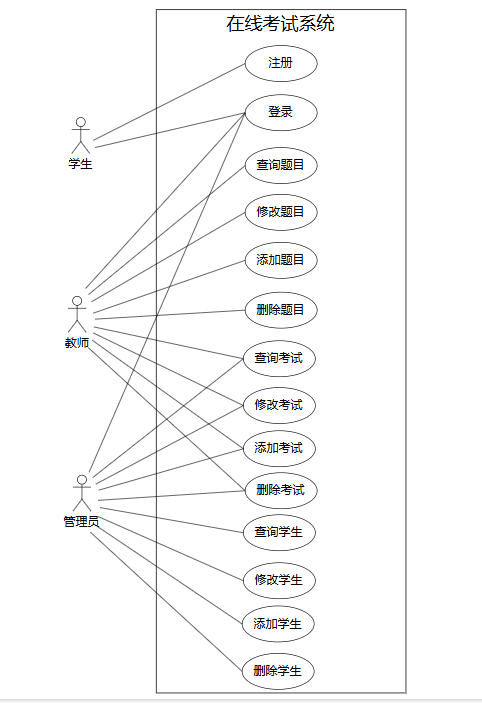
\includegraphics[width=0.4\linewidth]{use-case diagram.png}
    \end{figure}
\end{frame}
\begin{frame}{用例分析}
\framesubtitle{以UC008:添加题目为例}
\begin{itemize}
    \item \textbf{主要参与者}:教师  
    \item \textbf{涉众及其关注点}:教师希望能够向系统中添加新的题目信息  
    \item \textbf{前置条件}:教师已登录系统并进入题库管理界面  
    \item \textbf{成功保证}:系统能够安全、准确地存储新添加的题目信息至题库  
    \item \textbf{主成功场景}:教师输入新题目的各项信息(如题目内容、选项、答案等),系统保存信息并显示添加成功的消息  
\end{itemize}
\end{frame}
\begin{frame}{用例分析}
\framesubtitle{以UC008:添加题目为例}
\begin{itemize}
    \item \textbf{扩展}:如果输入的题目信息格式不正确或保存失败,系统应提示教师重新输入或联系技术支持  
    \item \textbf{特殊需求}:添加操作需要确保题目信息的唯一性和完整性  
    \item \textbf{技术与数据变元素}:输入新题目的信息(如题目内容、选项、答案等),点击添加按钮  
    \item \textbf{发生频率}:教师根据课程教学需求和题目变动情况定期进行题目信息的添加操作  
    \item \textbf{杂项}:系统应设计友好、易用的界面以便教师操作,同时保证操作流程清晰
\end{itemize}
\end{frame}
\section{系统设计}
\begin{frame}{交互设计}
    \begin{figure}
        \centering
        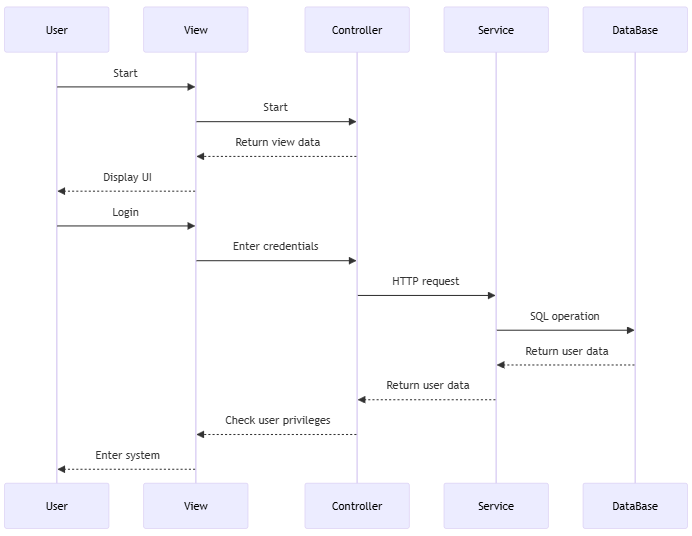
\includegraphics[width=0.7\linewidth]{sequence diagram (1).png}
    \end{figure}
\end{frame}
\begin{frame}{交互设计}
    \begin{figure}
        \centering
        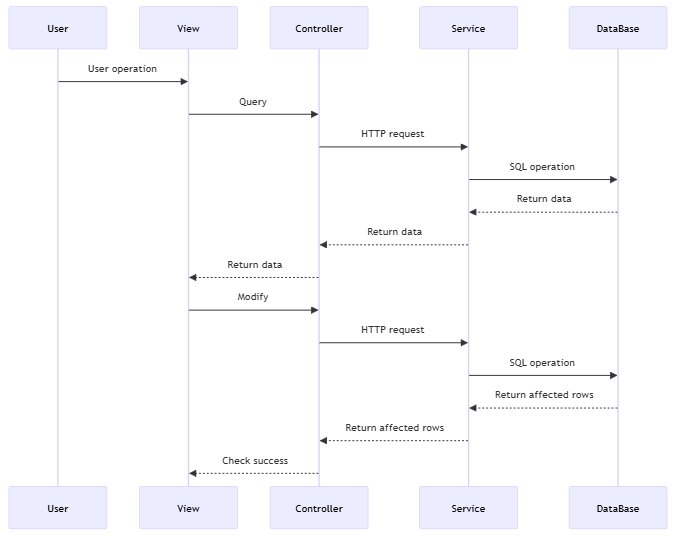
\includegraphics[width=0.7\linewidth]{sequence diagram (2).png}
    \end{figure}
\end{frame}
\begin{frame}{逻辑分层:View}
作用:
    \begin{itemize}
    \item 用户界面的展示和交互
    \item 接收用户的输入操作
    \item 将用户操作传递给控制器处理
    \end{itemize}
特征:
    \begin{itemize}
    \item HTML、Vue.js等前端技术。
    \item 负责呈现数据和收集用户输入。
    \item 不包含业务逻辑,专注于界面和用户交互。
    \end{itemize}
\end{frame}
\begin{frame}{逻辑分层:Controller}
作用:
    \begin{itemize}
    \item 处理用户的请求和操作。
    \item 调度和协调系统中的其他组件。
    \item 通常负责路由和请求转发。
    \end{itemize}
特征:
    \begin{itemize}
    \item Spring、Servlet等框架中的控制器。
    \item 接收来自视图层的请求并调用相应的服务层处理业务逻辑。
    \item 处理输入验证和参数校验,确保传递给服务层的数据有效性。
    \end{itemize}
\end{frame}
\begin{frame}{逻辑分层:Service}
作用:
    \begin{itemize}
    \item 执行业务逻辑和数据处理。
    \item 作为控制器和数据访问层(DAO层)之间的中介。
    \item 可以跨多个控制器共享。
    \end{itemize}
特征:
    \begin{itemize}
    \item Java类或者Spring的@Service注解类。
    \item 包含业务规则的实现,如数据处理、转换、验证等。
    \item 不直接与用户界面交互,而是接受控制器层传递的请求并返回处理结果。
    \end{itemize}
\end{frame}
\begin{frame}{逻辑分层:DataBase}
作用:
    \begin{itemize}
    \item 负责与数据库的交互。
    \item 执行数据的CRUD操作(创建、读取、更新、删除)。
    \item 提供持久化机制,确保数据的安全性和一致性。
    \end{itemize}
特征:
    \begin{itemize}
    \item DAO(Data Access Object)接口或者实现类。
    \item 使用JDBC、Hibernate、Spring Data等技术实现与数据库的通信。
    \item 负责处理数据库连接、事务管理、数据检索和更新等操作。
    \end{itemize}
\end{frame}
\begin{frame}{结构设计}
    \begin{figure}
        \centering
        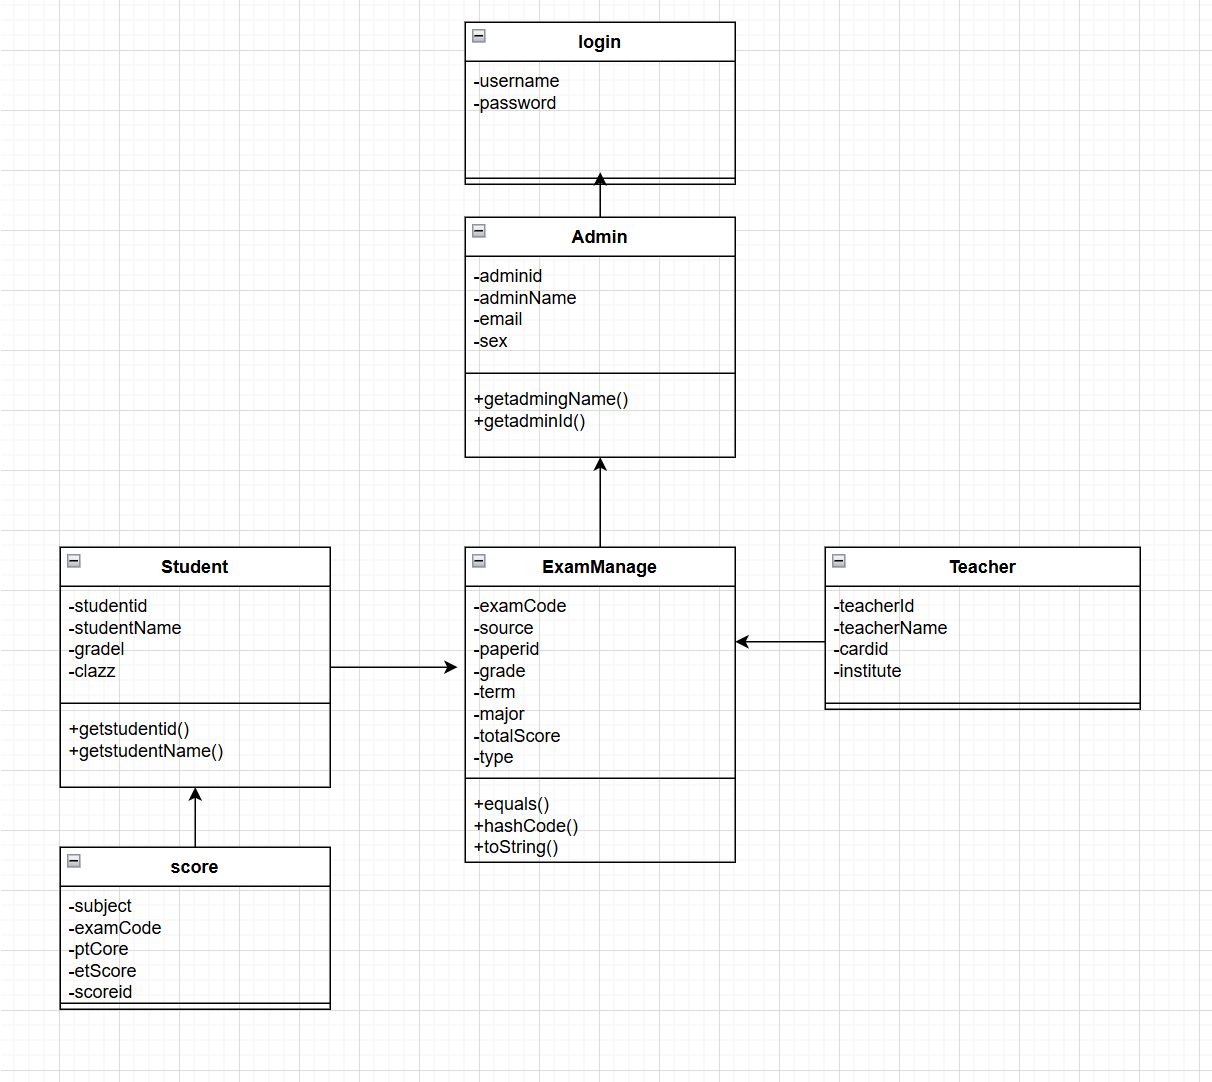
\includegraphics[width=0.65\linewidth]{class diagram.png}
    \end{figure}
\end{frame}
\begin{frame}{结构设计}
    \begin{figure}
        \centering
        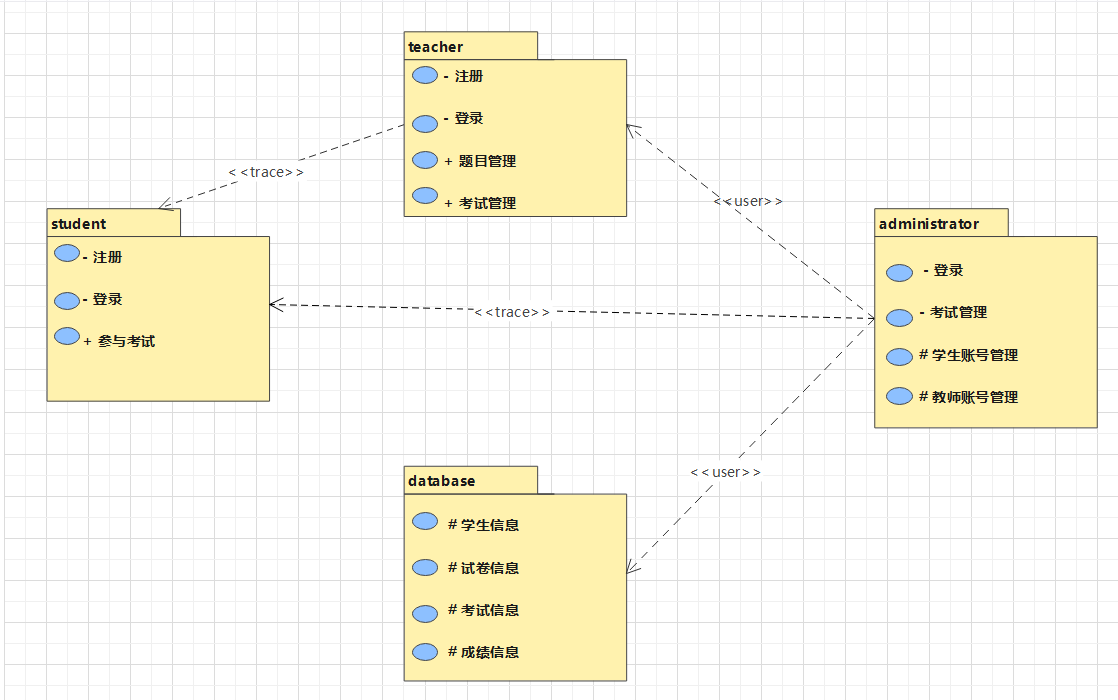
\includegraphics[width=0.85\linewidth]{package diagram.png}
    \end{figure}
\end{frame}
\begin{frame}{数据库设计}
    \begin{figure}
        \centering
        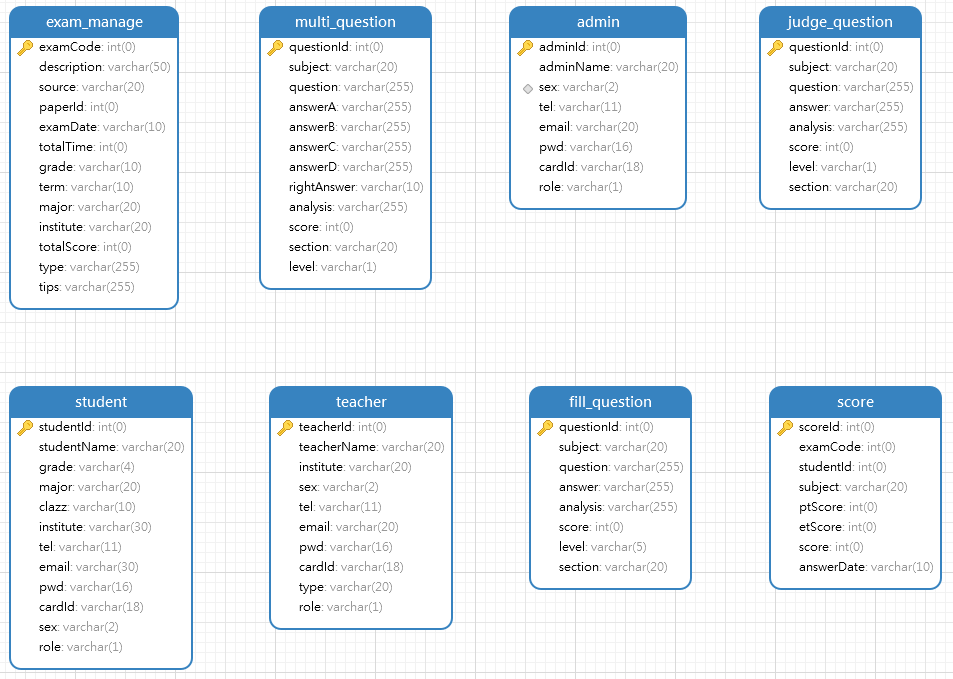
\includegraphics[width=0.85\linewidth]{database design.png}
    \end{figure}
\end{frame}
\section{软件运行效果}
\begin{frame}
    \centering\Huge{Thank You}
\end{frame}
\end{document}
